\documentclass[dvipdfmx,cjk,xcolor=dvipsnames,envcountsect,notheorems,12pt]{beamer}
% * 16:9 のスライドを作るときは、aspectratio=169 を documentclass のオプションに追加する
% * 印刷用の配布資料を作るときは handout を documentclass のオプションに追加する
%   (overlay が全て一つのスライドに出力される)

\usepackage{pxjahyper}% しおりの文字化け対策 (なくても良い)
\usepackage{amsmath,amssymb,amsfonts,amsthm,ascmac,cases,bm,pifont}
\usepackage{graphicx}
\usepackage{bussproofs}
\usepackage{url}
\usepackage{etex}

% スライドのテーマ
\usetheme{sumiilab}
% ベースになる色を指定できる
%\usecolortheme[named=Magenta]{structure}
% 数式の文字が細くて見難い時は serif の代わりに bold にしましょう
%\mathversion{bold}

%% ===============================================
%% スライドの表紙および PDF に表示される情報
%% ===============================================

%% 発表会の名前とか(省略可)
\session{平成26年度 卒業研究発表会}
%% スライドのタイトル
\title{MinCamlのK正規化の形式的検証}
%% 必要ならば、サブタイトルも
%\subtitle{}
%% 発表者のお名前
\author{B2TB2512 水野雅之}
%% 発表者の所属([] 内は短い名前)
\institute[東北大学 住井・松田研]{工学部 電気情報物理工学科\\住井・松田研究室}% 学部生
%\institute[東北大学 住井・松田研]{大学院情報科学研究科 情報基礎科学専攻\\住井・松田研究室}% 院生
%% 発表する日
\date{2016年3月11日}

%% ===============================================
%% 自動挿入される目次ページの設定(削除しても可)
%% ===============================================

%% section の先頭に自動挿入される目次ページ(削除すると、表示されなくなる)
\AtBeginSection[]{
\begin{frame}
  \frametitle{アウトライン}
  \tableofcontents[sectionstyle=show/shaded,subsectionstyle=show/show/hide]
\end{frame}}
%% subsection の先頭に自動挿入される目次ページ(削除すると、表示されなくなる)
\AtBeginSubsection[]{
\begin{frame}
  \frametitle{アウトライン}
  \tableofcontents[sectionstyle=show/shaded,subsectionstyle=show/shaded/hide]
\end{frame}}

%% 現在の section 以外を非表示にする場合は以下のようにする

%% \AtBeginSection[]{
%% \begin{frame}
%%   \frametitle{アウトライン}
%%   \tableofcontents[sectionstyle=show/hide,subsectionstyle=show/show/hide]
%% \end{frame}}
%% \AtBeginSubsection[]{
%% \begin{frame}
%%   \frametitle{アウトライン}
%%   \tableofcontents[sectionstyle=show/hide,subsectionstyle=show/shaded/hide]
%% \end{frame}}

%% ===============================================
%% 定理環境の設定
%% ===============================================

\setbeamertemplate{theorems}[numbered]% 定理環境に番号を付ける
\theoremstyle{definition}
\newtheorem{definition}{定義}
\newtheorem{axiom}{公理}
\newtheorem{theorem}{定理}
\newtheorem{lemma}{補題}
\newtheorem{corollary}{系}
\newtheorem{proposition}{命題}

%% ===============================================
%% ソースコードの設定
%% ===============================================

\usepackage{listings,jlisting}
%\usepackage[scale=0.9]{DejaVuSansMono}

\definecolor{DarkGreen}{rgb}{0,0.5,0}
% プログラミング言語と表示するフォント等の設定
\lstset{
  language={[Objective]Caml},% プログラミング言語
  basicstyle={\ttfamily\small},% ソースコードのテキストのスタイル
  keywordstyle={\bfseries},% 予約語等のキーワードのスタイル
  commentstyle={},% コメントのスタイル
  stringstyle={},% 文字列のスタイル
  frame=trlb,% ソースコードの枠線の設定 (none だと非表示)
  numbers=none,% 行番号の表示 (left だと左に表示)
  numberstyle={},% 行番号のスタイル
  xleftmargin=5pt,% 左余白
  xrightmargin=5pt,% 右余白
  keepspaces=true,% 空白を表示する
  mathescape,% $ で囲った部分を数式として表示する ($ がソースコード中で使えなくなるので注意)
  % 手動強調表示の設定
  moredelim=[is][\itshape]{@/}{/@},
  moredelim=[is][\color{red}]{@r\{}{\}@},
  moredelim=[is][\color{blue}]{@b\{}{\}@},
  moredelim=[is][\color{DarkGreen}]{@g\{}{\}@},
}

\newcommand{\keyword}[1]{\mathbf{#1}}
\newcommand{\LET}{\keyword{let}}
\newcommand{\REC}{\keyword{rec}}
\newcommand{\ARRAY}{\keyword{Array}}
\newcommand{\CREATE}{\keyword{create}}
\newcommand{\AND}{\keyword{and}}
\newcommand{\IN}{\keyword{in}}

%% ===============================================
%% 本文
%% ===============================================
\begin{document}
\frame[plain]{\titlepage}% タイトルページ

\begin{frame}
	\frametitle{研究概要}
	\LARGE MinCamlのK正規化をCoqで検証
	\begin{itemize}
		\item 余帰納的意味論
		\item ド・ブラン インデックス
		\item 半自動証明
	\end{itemize}
\end{frame}

\section*{アウトライン}

% 目次を表示させる(section を表示し、subsection は隠す)
\begin{frame}
  \frametitle{アウトライン}
  \tableofcontents[sectionstyle=show,subsectionstyle=hide]
\end{frame}

\section{研究背景}

\begin{frame}
	\frametitle{コンパイラのバグ}
	\LARGE コンパイラのバグは伝播

	\begin{itemize}
		\item UNIX初期のバックドア
	\end{itemize}

	\vfill

	{\Large
	\begin{tabular}{ccccc}
		\structure{正常なcc} & $\rightarrow$ & \alert{異常なcc} & & \\
																				& & \invisible<-1>{$\downarrow$} & & \\
		\structure{正常なlogin} & \invisible<-2>{$\rightarrow$} & \invisible<-1>{\alert{異常なcc}} & \invisible<-2>{$\rightarrow$} & \invisible<-2>{\alert{異常なlogin}}

	\pause
	\pause
\end{tabular}}

% バグの恐ろしさについては皆さんご存知と思いますが、
% コンパイラにバグがあると元のソースコードにバグが無くても誤ったバイナリが生成されてしまうので、
% コンパイラのバグと言うものは特に恐ろしいです。
% 典型的な例としては初期のUNIXに存在したバックドアでしょうか。
% ログインマネージャにバックドアを仕込むコンパイラを生成するコンパイラが頒布されたために、
% ソースコードには一切形跡を残さずにバックドアを仕込まれました。
\end{frame}

\begin{frame}
	\frametitle{現実の処理系}
	\LARGE 現実の処理系は複雑

	{\Large
	\begin{tabular}{ll}
		OCaml & 34万行 \\
		SML\# & 24万行 \\
		GCC & 1500万行
	\end{tabular}}

	\vfill
	素朴な検証では破綻
\end{frame}

\section{MinCaml}

\begin{frame}
	\frametitle{MinCaml}
	\LARGE 住井による教育用コンパイラ
	\begin{itemize}
		\item OCamlで2000行程度
		\item 非純粋な関数型言語
		\item 型推論
		\item 定数畳み込み等の最適化
	\end{itemize}
\end{frame}

\begin{frame}
	\frametitle{対象言語}
	\Large
	\[
	\begin{array}{l}
		M, N, e ::= \\
		\qquad \qquad \vdots\\
		\qquad \LET~\REC~x~y_1~\cdots~y_n=M~\IN~N\\
		\qquad M~N_1~\cdots~N_n\\
		\qquad (M_1,~\cdots~,M_n)\\
		\qquad \LET~(M_1,~\cdots~,M_n)=M~\IN~N\\
		\qquad \ARRAY.\CREATE~M~N\\
		\qquad M_1.(M_2)\\
		\qquad M_1.(M_2)\leftarrow M_3\\
	\end{array}
	\]
\end{frame}

\begin{frame}
	\frametitle{内部設計}
	\begin{figure}[htb]
		\centering
		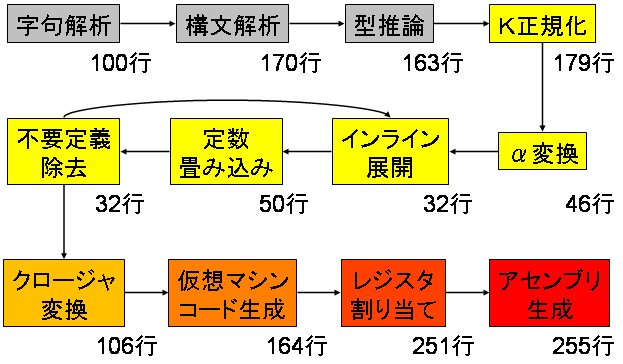
\includegraphics[width=12cm,clip]{mincaml.png}
	\end{figure}
\end{frame}

\begin{frame}
	\frametitle{K正規化}
	\LARGE 
	全ての部分式に名前を付ける

	\begin{columns}
		\begin{column}{0.5\textwidth}
			\begin{center}
				$a+b*c+d$
			\end{center}
		\end{column}
		\begin{column}{0.5\textwidth}
			\begin{center}
				\[
					\begin{array}{l}
						\LET~x = b * c~\IN \\
						\LET~y = a + x~\IN \\
						y + d
					\end{array}
				\]
			\end{center}
		\end{column}
	\end{columns}

	\vfill

	束縛の付け替えが伴う
\end{frame}

\section{意味論の定義}

\begin{frame}
	\frametitle{大ステップ意味論}
	\LARGE
	\begin{center}
	プログラム変換の検証に適する

	\vfill

	$\Updownarrow$

	\vfill

	無限ループとエラーの区別が困難
	\end{center}
\end{frame}

\begin{frame}
	\frametitle{例:型無しラムダ計算}
	\Large
	構文
	\begin{columns}
		\begin{column}{0.5\textwidth}
			\[
				\begin{array}{lcl}
					t & ::= & n \\
						& | & \lambda x.~t \\
						& | & t~t
				\end{array}
			\]
		\end{column}
		\begin{column}{0.5\textwidth}
			\[
				\begin{array}{lcl}
					v & ::= & n \\
						& | & \lambda x.~t \\
				\end{array}
			\]
		\end{column}
	\end{columns}

	\vfill

	意味論
	\begin{columns}
		\begin{column}{0.5\textwidth}
			\centering
			$n \Rightarrow n$
		\end{column}
		\begin{column}{0.5\textwidth}
			\centering
			$\lambda x.~t \Rightarrow \lambda x.~t$
		\end{column}
	\end{columns}

	\begin{prooftree}
		\AxiomC{$t_1 \Rightarrow \lambda x.~t_0$}
		\AxiomC{$t_2 \Rightarrow v_2$}
		\AxiomC{$[x \mapsto v_2]t_0 \Rightarrow v$}
		\TrinaryInfC{$t_1~t_2 \Rightarrow v$}
	\end{prooftree}
\end{frame}

\begin{frame}
	\frametitle{例:型無しラムダ計算}
	\begin{columns}
		\begin{column}{0.4\textwidth}
			{\LARGE エラー}
			{\Large \[ 0~0 \not \Rightarrow v \]}
			適用できる規則が無い
		\end{column}
		\begin{column}{0.6\textwidth}
			{\LARGE 無限ループ}
			{\Large \[ ~(\lambda x.xx)(\lambda x.xx) \not \Rightarrow v \]}
			有限回の規則適用で導出できない
		\end{column}
	\end{columns}

	\vfill

	\begin{center}
		{\LARGE 区別できない}
	\end{center}
\end{frame}

\begin{frame}
	\frametitle{余帰納的大ステップ意味論}
	\LARGE
	余帰納的定義
	\begin{columns}
		\begin{column}{0.3\textwidth}
			\begin{prooftree}
				\AxiomC{$t_1 \mathop{\Rightarrow}\limits^{\infty}$}
				\UnaryInfC{$t_1~t_2 \mathop{\Rightarrow}\limits^\infty$}
			\end{prooftree}
		\end{column}
		\begin{column}{0.7\textwidth}
			\begin{prooftree}
				\AxiomC{$t_1 \Rightarrow v_1$}
				\AxiomC{$t_2 \mathop{\Rightarrow}\limits^\infty$}
				\BinaryInfC{$t_1~t_2 \mathop{\Rightarrow}\limits^\infty$}
			\end{prooftree}
		\end{column}
	\end{columns}

	\begin{prooftree}
		\AxiomC{$t_1 \Rightarrow \lambda x.~t_0$}
		\AxiomC{$t_2 \Rightarrow v_2$}
		\AxiomC{$[x \mapsto v_2]t_0 \mathop{\Rightarrow}\limits^\infty$}
		\TrinaryInfC{$t_1~t_2 \mathop{\Rightarrow}\limits^\infty$}
	\end{prooftree}
\end{frame}

\begin{frame}
	\frametitle{余帰納的大ステップ意味論}
	\LARGE
	\begin{columns}
		\begin{column}{0.4\textwidth}
			エラー
			\[ 0~0 \not {\mathop{\Rightarrow}\limits^\infty} \]
			{\normalsize 適用できる規則がない}
		\end{column}
		\begin{column}{0.6\textwidth}
			無限ループ
			\[ (\lambda x.x x)(\lambda x.x x) \mathop{\Rightarrow}\limits^\infty \]
			{\normalsize 無限回の規則適用を許す}
		\end{column}
	\end{columns}

	\vfill

	\begin{center}
		区別できる
	\end{center}
\end{frame}

\section{束縛の表現}

\begin{frame}
	\frametitle{名前による表現}
	\LARGE $\alpha$等価性の議論が面倒
	\[ \lambda x.\lambda y.~x \simeq \lambda a.\lambda b.~a \]

	\vfill

	捕獲が起こりうる
	\[ 
		\begin{array}{lcl}
			[x \mapsto z](\lambda z.~x) & = & \lambda w.~z \\
																	& \not = & \lambda z.~z
		\end{array}
	\]
\end{frame}

\begin{frame}
	\frametitle{ド・ブラン インデックス}
	\LARGE
	何番目の束縛かで変数を表現
	\begin{columns}
		\begin{column}{0.5\textwidth}
			\[ \lambda x. \lambda y. \lambda z.~x z (y z) \]
		\end{column}
		\begin{column}{0.5\textwidth}
			\[ \lambda. \lambda. \lambda.~2~0~(1~0) \]
		\end{column}
	\end{columns}

	\vfill

	$\alpha$等価な式は文面上も等価
	\begin{columns}
		\begin{column}{0.5\textwidth}
			\[ \lambda x.\lambda y.~x \]
			\[ \lambda a.\lambda b.~a \]
		\end{column}
		\begin{column}{0.5\textwidth}
			\[ \lambda.\lambda.~1 \]
		\end{column}
	\end{columns}

	\vfill

	捕獲も回避できる
\end{frame}

\begin{frame}
	\frametitle{シフト}
	\LARGE 自由変数のインデックスをずらす
	\[\uparrow^d t \]

	束縛の付け替え
	\begin{columns}
		\begin{column}{0.5\textwidth}
			\[ \lambda x.~x \]
		\end{column}
		\begin{column}{0.5\textwidth}
			\[ \lambda.~1 \]
		\end{column}
	\end{columns}

	\vfill

	\begin{columns}
		\begin{column}{0.5\textwidth}
			\[ \lambda x.\lambda y.~x \]
		\end{column}
		\begin{column}{0.5\textwidth}
			\[
				\begin{array}{l}
					\lambda.\lambda.~\uparrow^1 0 \\
					= \lambda. \lambda.~1
				\end{array}
			\]
		\end{column}
	\end{columns}
\end{frame}

\begin{frame}[fragile]
	\frametitle{K正規化の実装}
\begin{lstlisting}[frame=none]
Fixpoint knormal e :=
  match e with
  | Exp.Var x => Var x
  | Exp.Abs e => Abs (knormal e)
  | Exp.App e1 e2 =>
      Let (knormal e1)
        (Let (shift 1 (knormal e2))
          (App 1 0))
  end.
\end{lstlisting}
\end{frame}

\section{正当性の検証}

\begin{frame}[fragile]
	\frametitle{コンパイラの検証}
	\LARGE 言語拡張のたび全ての証明を修正
	\begin{columns}
		\begin{column}{0.5\textwidth}
\begin{lstlisting}[frame=none]
Inductive t :=
  | Var : nat -> t
$\vdots$
Proof.
  intros t.
  induction t.
  Case "Var".
\end{lstlisting}
		\end{column}
		\begin{column}{0.5\textwidth}
\begin{lstlisting}[frame=none]
Inductive t :=
  @r{| Int : Z -> t}@
  | Var : nat -> t
$\vdots$
Proof.
  intros t.
  induction t.
  @r{Case "Nat".}@
    $\vdots$
  Case "Var".
\end{lstlisting}
		\end{column}
	\end{columns}
\end{frame}

\begin{frame}[fragile]
	\frametitle{Coqの証明自動化機能}
	\LARGE 構文の違いを自動証明で吸収

	\vfill

\begin{lstlisting}[frame=none]
Lemma shift_0 : forall e c,
  shift c 0 e = e.
Proof.
  intros e.
  induction e; intros ?; simpl;
    f_equal;
    solve [ apply shift_var_0 | eauto ].
Qed.
\end{lstlisting}
\end{frame}

\begin{frame}
	\frametitle{言語の拡張}
	\LARGE 四則演算、if等を追加
	\begin{center}
		\Large 
		\begin{tabular}{|l||l|l|}
			\hline
			 & 構文の種類 & 証明の行数 \\
			\hline
			\hline
			拡張前 & 3 & 110 \\
			\hline
			拡張後 & 20 & 141 \\
			\hline
		\end{tabular}
	\end{center}

	\vfill

	高い再利用性を示した
\end{frame}

\section{結論}

\begin{frame}
	\frametitle{結論}
	\Large K正規化をCoqで検証できた
	\begin{itemize}
		\item ド・ブラン インデックス、\\余帰納的大ステップ意味論の採用で証明が簡潔に
		\item 証明自動化による再利用性の高い証明
	\end{itemize}
\end{frame}

\begin{frame}
	\frametitle{今後の課題}
	\Large さらに言語を拡張し、MinCamlと同等に
	\begin{itemize}
		\item タプルや複数引数の関数
		\item 配列
		\item 外部関数呼び出し
	\end{itemize}

	\vfill

	K正規化以外の検証
\end{frame}

\end{document}
